\documentclass[12pt, a4paper]{article}
\usepackage[a4paper, includeheadfoot, mag=1000, left=2cm, right=1.5cm, top=1.5cm, bottom=1.5cm, headsep=0.8cm, footskip=0.8cm]{geometry}
% Fonts
\usepackage{fontspec, unicode-math}
\setmainfont[Ligatures=TeX]{CMU Serif}
\setmonofont{CMU Typewriter Text}
\usepackage[english, russian]{babel}
% Indent first paragraph
\usepackage{indentfirst}
\setlength{\parskip}{5pt}
% Diagrams
\usepackage{graphicx}
\usepackage{float}
% Page headings
\usepackage{fancyhdr}
\pagestyle{fancy}
\renewcommand{\headrulewidth}{0pt}
\setlength{\headheight}{16pt}
%\newfontfamily\namefont[Scale=1.2]{Gloria Hallelujah}
\fancyhead{}
% Python
\usepackage{pythontex}


\usepackage{listings}
\lstdefinestyle{lablisting}{
  basicstyle=\scriptsize\ttfamily,
  numbers=left,
  stepnumber=1,
  otherkeywords={EOF, O\_RDONLY, STDIN\_FILENO, STDOUT\_FILENO, STDERR\_FILENO},
  numbersep=10pt,
  showspaces=false,
  showstringspaces=false
}

\graphicspath{ {images/} }

\newcommand{\specialcell}[2][l]{%
  \begin{tabular}[#1]{@{}l@{}}#2\end{tabular}}

\newcommand{\bandwidthEntry}[1]{
  \hline
  \multicolumn{2}{|c|}{Пропускная способность: #1 Mbps} \\
  \hline
  Частота основной гармоники сигнала \texttt{11111...} & 0 Гц \\
  Верхняя граница частот в передаваемом сообщении & \py{int(max_mult * f_0[#1])} Гц \\
  Нижняя граница частот в передаваемом сообщении & \py{int(f_0[#1] / max_count)} Гц \\
  Необходимая полоса пропускания & \py{int(f_0[#1] / max_count)} : \py{int(max_mult * f_0[#1])} Гц \\
}

\begin{document}

\begin{pycode}
from utils import *
\end{pycode}

% Title page
\begin{titlepage}
\begin{center}

\textsc{Национальный исследовательский университет ИТМО\\[4mm]
Факультет программной инженерии и компьютерной техники}
\vfill
\textbf{Учебно-исследовательская работа №1\\[4mm]
по дисципение Сети ЭВМ и телекоммуникации\\[16mm]
}
\begin{flushright}
Студент: Саржевский Иван
\\[2mm]Группа: P3302
\end{flushright}
\vfill
г. Санкт-Петербург\\[2mm]
2020 г.

\end{center}
\end{titlepage}

\tableofcontents
\newpage

\section{Цель}

Изучение методов логического и физического кодирования, используемых в цифровых
сетях передачи данных.

\section{Задание}

Выполнить логическое и физическое кодирование исходного сообщения в соответствии
с заданными методами кодирования, провести сравнительный анализ рассматриваемых
методов кодирования, выбрать и обосновать наилучший метод для передачи исходного
сообщения.

\section{Формирование сообщения}

\begin{tabular}{ l l }
  \textit{Сообщение:} & \texttt{Саржевский И.А.} \\
  \textit{Hex-код:} & \texttt{D1 E0 F0 E6 E5 E2 F1 EA E8 E9 20 C8 2E C0 2E} \\
  \textit{Bin-код:} & \specialcell[l]{
    \texttt{11010001 11100000 11110000 11100110 11100101 11100010 11110001} \\
    \texttt{11101010 11101000 11101001 00100000 11001000 00101110 11000000} \\
    \texttt{00101110}
  } \\
  \textit{Длина:} & 15 байт (120 бит)
\end{tabular}

\section{Физическое кодирование}

\subsection{Выделение основной частоты}

Определим частоту основной гармоники бесконечного сигнала \texttt{10101010...}
как базовую частоту $f_0$. В таком случае, частоту основной гармоники сигнала
с повторением произвольного количества нулей и единиц удобно представить в
виде $f = f_0 / x$, где $x$ - длина последовательности нулей и единиц (например,
очевидно что частота основной гармоники сигнала \texttt{110011001100...} равна
$f_0 / 2$).

Введение такой переменной позволяет нам записать ряд Фурье для бесконечного
сигнала с повторением произвольного количества нулей и единиц таким образом:

$$\sum_y (A_0 / y) \sin (2 \pi \frac{y f_0}{x} t)$$

, где $y \in \{ 1, 3, 5, 7 \}$, а $x$ - длина периода повторяющихся символов.

Определим $f_0$ для разных значений пропускной способности. Она будет равна
единице, деленной на период основной гармоники, равный времени передачи двух
бит сообщения. Таким образом, для пропускной способности $x$:

\newpage

\noindent $B_t = 1 / x$ \\
$T_0 = 2 B_t$ \\
$f_0 = 1 / T_0$ \\

\begin{tabular}{ c | c }
  Пропускная способность, Mbps & Базовая частота $f_0$, Гц \\
  10 & $0.5 * 10^7$ \\
  100 & $0.5 * 10^8$ \\
  1000 & $0.5 * 10^9$
\end{tabular}

\subsection{Потенциальный код NRZ}

\begin{figure}[h]
  \begin{center}
    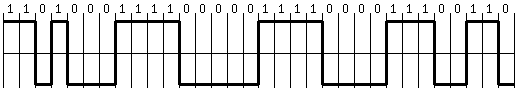
\includegraphics{nrz}
    \caption{Кодирование первых четырех байт потенциальным кодом NRZ}
  \end{center}
\end{figure}

\begin{pycode}
nrz_string = '11010001111000001111000011100110111001011110001011110001111010'\
  '1011101000111010010010000011001000001011101100000000101110'
[max_count, max_char] = longest_substing(nrz_string)
max_mult = 7
\end{pycode}

Из диаграммы легко понять, что $T_{min}$ достигается при кодировании чередующихся
сигналов, из чего следует, что $T_{min} = T_0$ и $f_{max} = f_0$. Для определения
$T_{max}$ найдем участок с минимальным чередованием. Для данного вида кодирования
такой участок достигается при передаче последовательности из \py{max_count}
символов \texttt{\py{max_char}},
следовательно $T_{max} = \py{max_count} T_0$, а $f_{min} = \frac{f_0}{\py{max_count}}$.

Разложение в ряд Фурье для сигнала представляющего из себя последовательность
чередующихся единиц и нулей будет иметь вид:

$$A_0 \sin(2 \pi f_0 t) + (A_0 / 3) \sin(2 \pi 3 f_0 t) +
  (A_0 / 5) \sin(2 \pi 5 f_0 t) + (A_0 / 7) \sin(2 \pi 7 f_0 t)$$

Аналогичное разложение для сигнала с чередующимися последовательностями из
\py{max_count} единиц и нулей будет иметь вид:

$$A_0 \sin(2 \pi \frac{f_0}{\py{max_count}} t) + (A_0 / 3) \sin(2 \pi \frac{3 f_0}{\py{max_count}} t) +
  (A_0 / 5) \sin(2 \pi \frac{5 f_0}{\py{max_count}} t) + (A_0 / 7) \sin(2 \pi \frac{7 f_0}{\py{max_count}} t)$$

Получаем спектр частот $\frac{f_0}{\py{max_count}}...7 f_0$.

\newpage

\begin{tabular}{| c | c |}
  \bandwidthEntry{10}
  \bandwidthEntry{100}
  \bandwidthEntry{1000}
  \hline
\end{tabular}

\subsubsection*{Определение среднего значения чаcтоты передаваемого сообщения}

\begin{pycode}
occurrence = get_occurrence_counts(nrz_string)
build_occurrence_table(occurrence)
\end{pycode}

\begin{pycode}
mes_len = len(nrz_string)
print(get_f_mean_math(occurrence, mes_len))
get_f_mean_table(occurrence, mes_len)
\end{pycode}


\end{document}
